\def \phi {1.617}
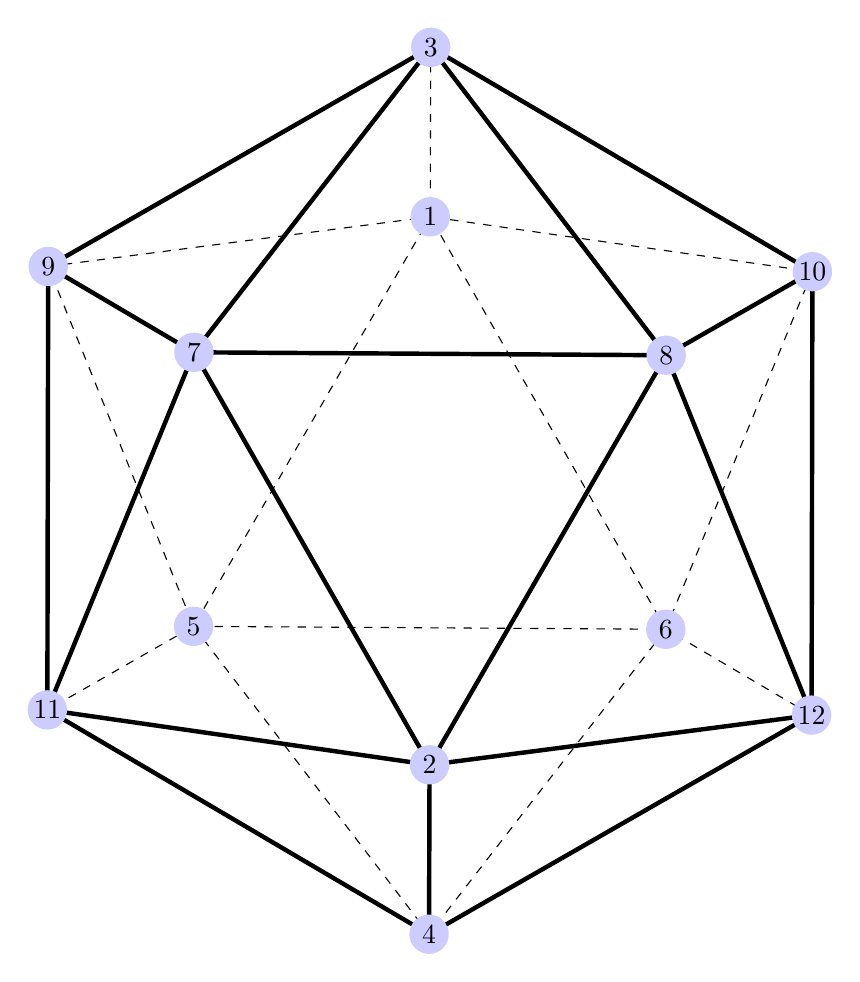
\begin{tikzpicture}[
    x={(-0.86in, -0.5in)}, y = {(0.86in, -0.5in)}, z = {(0, 1in)},
    rotate = 22,
    scale = 0.6,
    every node/.style = {
      circle, fill = blue!20, inner sep = 0pt, minimum size = 0.5cm
    },
    foreground/.style = { ultra thick },
    background/.style = { dashed }
  ]
  \coordinate (9) at (0, -\phi*\phi,  \phi);
  \coordinate (8) at (0,  \phi*\phi,  \phi);
  \coordinate (12) at (0,  \phi*\phi, -\phi);
  \coordinate (5) at (0, -\phi*\phi, -\phi);
  \coordinate (7) at ( \phi, 0,  \phi*\phi);
  \coordinate (3) at (-\phi, 0,  \phi*\phi);
  \coordinate (6) at (-\phi, 0, -\phi*\phi);
  \coordinate (4) at ( \phi, 0, -\phi*\phi);
  \coordinate (2) at ( \phi*\phi,  \phi, 0);
  \coordinate (10) at (-\phi*\phi,  \phi, 0);
  \coordinate (1) at (-\phi*\phi, -\phi, 0);
  \coordinate (11) at ( \phi*\phi, -\phi, 0);

  \draw[foreground] (10) -- (3) -- (8) -- (10) -- (12) -- (8);
  \draw[foreground] (4) -- (12) -- (2) -- (4) -- (11) -- (2);
  \draw[foreground] (9) -- (3) -- (7) -- (9) -- (11) -- (7);
  \draw[foreground] (7) -- (8) -- (2) -- cycle;
  \draw[background] (12) -- (6) -- (10) -- (1) -- (6) -- (5) -- (1)
    -- (9) -- (5) -- (11);
  \draw[background] (5) -- (4) -- (6);
  \draw[background] (3) -- (1);
  \foreach \n in {1,...,12}
    \node at (\n) {\n};
\end{tikzpicture}